\documentclass{standalone}
\usepackage{tikz}
\usepackage{ctex,siunitx}
\setCJKmainfont{Noto Serif CJK SC}
\usepackage{tkz-euclide}
\usepackage{amsmath}
\usetikzlibrary{patterns, calc}
\usetikzlibrary {decorations.pathmorphing, decorations.pathreplacing, decorations.shapes,}

\begin{document}
\small
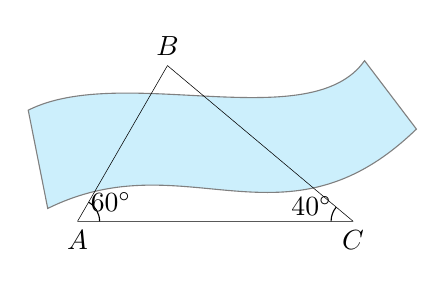
\begin{tikzpicture}[>=stealth,scale=0.7]
  \tkzSetUpPoint[fill=black]
  % \useasboundingbox(-1,-0.75)rectangle(3.7,1.4);
  \tkzDefPoints{0/0/A, 5/0/C}
  \tkzDefShiftPoint[A](60:1){A'}
  \tkzDefShiftPoint[C](140:1){C'}
  \tkzInterLL(A,A')(C,C')\tkzGetPoint{B}
  \fill[cyan!20,draw=gray](-0.895, 2.016)..controls( 0.811, 2.874)and( 4.229, 1.524)..( 5.207, 2.914)--( 6.148, 1.673)..controls( 3.760,-0.640)and( 1.973, 1.471)..(-0.541, 0.233)--cycle;
  \tkzDrawPolygon(A,B,C)
  \tkzLabelPoints(A,C)
  \tkzMarkAngle[size=0.4](C,A,B)
  \tkzLabelAngle[pos=0.7](C,A,B){\ang{60}}
  \tkzMarkAngle[size=0.4](B,C,A)
  \tkzLabelAngle[pos=0.8](B,C,A){\ang{40}}
  \tkzLabelPoints[above](B)
\end{tikzpicture}
\end{document}